% !TEX root =../../main.tex
%%
%% Capítulo 4: Problema
%%

\mychapter{Problema}
\label{Cap:Problema}

Aqui você deve especificar o seu problema (de forma muito formal). Coloque a matemática (ou descreva a problemática) do problema. Use e abuse de Definições, Teoremas, Proposições e Provas. Descreva a sua solução (matemática) para o problema em questão, como você resolve o problema.
Pode ser descritivo, mas provando que funciona matematicamente (ou formalmente).

\section{Elementos flutuantes}
\label{Sec:flutuantes}

Uma das maiores dificuldades na edição de textos de qualidade é o
posicionamento dos elementos gráficos: figuras, gráficos e
tabelas. Como estes elementos muitas vezes são grandes, aparece o
dilema sobre o que fazer quando uma quebra de página deveria acontecer
no meio do elemento. Há duas possibilidades:
\begin{enumerate}
\item O autor informa exatamente onde o elemento gráfico deve ficar no
texto, evitando que quebras de páginas aconteçam no meio de um
elemento. O problema com esta abordagem é que todo o trabalho de
posicionamento pode ser perdido caso se inclua ou se exclua algum
texto ou elemento.
\item O editor de texto posiciona os elementos gráficos de forma a não
deixar espaços em branco nas páginas. Estes elementos que podem ser
posicionados pelo editor são conhecidos como \emph{elementos
flutuantes}. O problema com esta abordagem é que o posicionamento
adotado pode não corresponder às expectativas do autor.
\end{enumerate}

O \LaTeX\ oferece as duas possibilidades de posicionamento. Este
capítulo apresenta exemplos de inclusão de elementos gráficos no
texto, bem como algumas ferramentas externas ao \LaTeX\ que podem ser
utilizadas para gerá-los.

Para caracterizar uma parte do texto como sendo flutuante, ela deve ser
delimitada por \verb|\begin{figure}| e \verb|\end{figure}| ou por
\verb|\begin{table}| e \verb|\end{table}|. Apesar do que os nomes
sugerem, nada obriga que o ambiente \texttt{figure} seja usado para
delimitar figuras ou que o ambiente \texttt{table} seja usado para
delimitar tabelas, embora esta seja a escolha quase sempre
adotada. Estes dois ambientes são praticamente equivalentes, com as
seguintes diferenças:
\begin{itemize}
\item os dois ambientes usam contadores diferentes para numerar os
elementos flutuantes;
\item os ambientes \texttt{figure} serão incluídos na
\texttt{listoffigures}, enquanto os ambientes \texttt{table} serão
incluídos na \texttt{listoftables};
\item as legendas (\texttt{caption}'s) dos ambientes \texttt{figure}
serão precedidas da palavra ``Figura \dots'', enquanto as legendas dos
ambientes \texttt{table} serão precedidas da palavra ``Tabela \dots''.
Estas duas palavras podem ser alteradas pelo autor.
\end{itemize}
Para ilustrar o fato de que estes ambientes podem conter virtualmente
qualquer coisa, a figura~\ref{Fig:textoflutuante} contém um texto que
foi tornado flutuante por ser incluído em um ambiente \texttt{figure}
e as tabelas \ref{Tab:equacaoflutuante} e \ref{Tab:equacaoflutuante2}
contêm expressões matemáticas flutuantes, incluídas em um ambiente
\texttt{table}. A tabela (\texttt{table}) \ref{Tab:submultilinhas} na
página \pageref{Tab:submultilinhas} também não contém uma tabela no
sentido estrito do termo, mas sim uma linha de texto formada por duas
\texttt{minipage}'s separadas por um espaço horizontal. A primeira
\texttt{minipage} contém um trecho de código fonte e a segunda, o
resultado produzido (uma expressão matemática multialinhada).

\begin{figure}[tbp]
\caption{Trecho de \emph{Os Lusíadas}, de Luis de Camões}
\label{Fig:textoflutuante}
% hrule - linha horizontal
\hrule
% As minipage's são muito úteis para se colocar duas coisas na mesma linha
\begin{minipage}{0.45\linewidth}
% flushleft - alinha à esquerda
\begin{flushleft}
As armas e os barões assinalados\\
Que da ocidental praia lusitana\\
Por mares nunca dantes navegados\\
Passaram ainda além da Trapobana\\
Em perigos e guerras esforçados\\
Mais do que prometia a força humana\\
Entre gente remota edificaram\\
Novo reino, que tanto sublimaram
\end{flushleft}
\end{minipage}
\hfill
\begin{minipage}{0.45\linewidth}
% flushright - alinha à direita
\begin{flushright}
E também as memórias gloriosas\\
Daqueles reis que foram dilatando\\
A Fé, o Império, as terras viciosas\\
De África e Ásia andaram devastando,\\
E aqueles que por obras valerosas\\
Se vão da lei da morte libertando:\\
Cantando espalharei por toda parte,\\
Se a tanto me ajudar o engenho e arte.
\end{flushright}
\end{minipage}
\hrule
\end{figure}

\begin{table}[bp]
% As minipage's são muito úteis para se colocar duas coisas na mesma linha
\begin{minipage}[b]{0.45\linewidth}
\begin{center}
\[
ax^2 + bx + c = 0
\]
\end{center}
\caption{Equação de segundo grau}
\label{Tab:equacaoflutuante}
\end{minipage}
\hfill
\begin{minipage}[b]{0.50\linewidth}
\begin{center}
\[
x = \frac{-b\pm\sqrt{b^2-4ac}}{2a}
\]
\end{center}
\caption{Raízes da equação da tabela~\ref{Tab:equacaoflutuante}}
\label{Tab:equacaoflutuante2}
\end{minipage}
\end{table}

É importante ressaltar que o que é numerado é o \texttt{caption} e não
a \texttt{figure} ou a \texttt{table}. Portanto, o \texttt{label} deve
ser colocado sempre após o \texttt{caption} ao qual ele se
refere. Conforme ilustram as tabelas \ref{Tab:equacaoflutuante} e
\ref{Tab:equacaoflutuante2}, uma mesma \texttt{figure} ou
\texttt{table} pode ter mais de um ou nenhum \texttt{caption}.
O \texttt{caption} pode ser colocado antes do conteúdo flutuante, como
na figura \ref{Fig:textoflutuante}, ou depois, como nas tabelas
\ref{Tab:equacaoflutuante} e \ref{Tab:equacaoflutuante2}. Nos
documentos do PPgEEC, o padrão é sempre posicionar o \texttt{caption}
abaixo das figuras e das tabelas.

\subsection{Posicionamento dos elementos flutuantes}
\label{Sec:posicionamento}

Em cada \verb|\begin{figure}| ou \verb|\begin{table}| pode-se incluir
um parâmetro opcional com as opções de posicionamento para este
elemento flutuante. Parâmetros adicionais de comandos \LaTeX\ são
sempre fornecidos entre colchetes \texttt{[]}, enquanto os parâmetros
obrigatórios aparecem entre chaves \verb|{}|. As opções disponíveis
incluem as seguintes:
\begin{itemize}
\item[\tt h] O elemento pode ser posicionado na mesma posição em que ele
aparece no código fonte do texto.
\item[\tt t] O elemento pode ser posicionado no topo de uma página.
\item[\tt b] O elemento pode ser posicionado no fim de uma página.
\item[\tt p] O elemento pode ser incluído em uma página formada só por
flutuantes.
\item[\tt !] Normalmente o \LaTeX\ faz algumas considerações de ordem
estética no posicionamento dos flutuantes, o que às vezes faz com que
alguns elementos sejam posicionados muito longe de onde são citados,
principalmente se você não incluir a opção \texttt{p}. Para fazer com
que as considerações estéticas não sejam levadas em conta para um dado
elemento, inclua a opção \texttt{!}.
\end{itemize}

\section{Tabelas em \LaTeX}
\label{Sec:tabelas}

Tabelas são construídas com comandos próprios do \LaTeX, notadamente o
ambiente \texttt{tabular}. Nada obriga a que o ambiente
\texttt{tabular} esteja sempre posicionado em um elemento
flutuante. Se você quiser impor que uma tabela fique obrigatoriamente
em uma determinada posição do texto, basta não colocar o
\texttt{tabular} dentro de um \texttt{table}. Tabelas podem até ser
incluídas no meio de uma frase.  Por exemplo, eu posso dizer que se um
jogo da velha está na configuração \textsf{\tiny\begin{tabular}{c|c|c}
x & & x \\ \hline & & o \\ \hline x & o & \end{tabular}} e se o
jogador ``\textsf{x}'' sabe jogar, então o jogador ``\textsf{o}'' irá
perder, independentemente da jogada que faça.

O ambiente \texttt{tabular} tem um parâmetro obrigatório que indica o
número de colunas da tabela e o posicionamento dos objetos em cada
coluna. Por exemplo, uma tabela criada com \verb|\begin{tabular}{lcr}|
terá três colunas; o texto será alinhado à esquerda na primeira
coluna, centralizado na segunda e alinhado à direita na
terceira. Podem ser incluídos objetos que ocupam mais de uma linha
(comando \texttt{multirow}) ou mais de uma coluna (comando
\texttt{multicolumn}). Neste último caso, também é possível mudar o
alinhamento do texto. Exemplos podem ser vistos nas tabelas
\ref{Tab:multilinhas} e \ref{Tab:submultilinhas}, na
página~\pageref{Tab:multilinhas}.

Com o pacote \texttt{tabularx}, além das opções normais de
posicionamento de colunas (\texttt{lcr}), pode-se incluir
automaticamente um texto qualquer antes de cada elemento da coluna
(\verb|>{}|). Este recurso foi utilizado nas tabelas
\ref{Tab:multilinhas} e \ref{Tab:submultilinhas} para fazer
com que todos os textos de algumas colunas fossem automaticamente
escritos na fonte \texttt{tt}. Além disso, podem-se criar colunas de
largura fixa e/ou de largura que se ajustam para que a tabela ocupe
toda a largura desejada, além do estilo tradicional de coluna que
assume a largura suficiente para conter seus elementos. Exemplos de
colunas com diferentes larguras e alinhamentos podem ser vistos na
tabela \ref{Tab:larguracolunas}.

\begin{table}[htbp]
\begin{tabularx}{\linewidth}{|p{3cm}|X|l|} \hline
COLUNA p & COLUNA X & COLUNA l \\ \hline
Largura fixa (não depende do conteúdo) &
Expandível &
Ajustável \\ \hline
Alinhada no topo &
Alinhada à esquerda &
Alinhada à esquerda \\ \hline
\end{tabularx}
\\[0.5cm]
\begin{tabularx}{\linewidth}{|b{3cm}|C|r|} \hline
COLUNA b & COLUNA C (ver \texttt{comandos.tex}) & COLUNA r \\ \hline
Largura fixa (não depende do conteúdo) &
Expandível &
Ajustável \\ \hline
Alinhada na base &
Centralizada &
Alinhada à direita \\ \hline
\end{tabularx}
\caption{Tabelas com colunas de diferentes larguras e alinhamentos}
\label{Tab:larguracolunas}
\end{table}

\section{Figuras em \LaTeX}
\label{Sec:figuras}

As figuras (imagens, desenhos, gráficos, etc.) devem ser produzidas
por ferramentas externas ao \LaTeX, salvas em um arquivo e inseridas
no texto usando o comando \texttt{includegraphics}. Da mesma forma
que as tabelas, as figuras podem ser flutuantes, caso sejam
inseridas dentro de um ambiente \texttt{figure}, ou ter uma posição
fixa no texto (como aqui: 
\includegraphics{textuais/04-problema/figuras/eu.eps}).

O formato em que você deve salvar os arquivos das figuras para que
possa incluí-las no texto depende de como você pretende compilar
o código fonte:
\begin{itemize}
\item se o texto vai ser compilado com \texttt{latex}, todos os
arquivos devem estar no formato EPS (\emph{Encapsulated PostScipt});
\item se o texto vai ser compilado com \texttt{pdflatex}, os
arquivos devem estar nos formatos PDF ou JPEG (outros formatos são
aceitos, mas estes são os recomendáveis).
\end{itemize}
É aconselhável que você não inclua a terminação no nome do arquivo que
é parâmetro para o comando \texttt{includegraphics}. Isto porque, de
acordo com a forma como o texto está sendo compilado, o \LaTeX\
acrescenta a terminação adequada. Por exemplo, caso seu texto inclua o
comando \verb|
\includegraphics{eu}|, o \LaTeX\ procurará o arquivo
\texttt{eu.eps} caso esteja sendo chamado via \texttt{latex} ou um dos
arquivos \texttt{eu.pdf} ou \texttt{eu.jpg} caso esteja sendo chamado
via \texttt{pdflatex}.

As figuras podem ser divididas em dois grandes grupos:
\begin{itemize}
\item As imagens e fotos, que normalmente correspondem a visões reais
do mundo e são obtidas por câmeras digitais ou
assemelhados. Caracterizam-se por conterem grandes quantidades de
nuances, texturas e cores.
\item As figuras sintéticas, normalmente produzidas utilizando
\emph{softwares} dedicados. Geralmente contêm figuras geométricas
(linhas, quadrados, etc.), textos e poucas cores e texturas. Neste
grupo, para efeito de discussão das ferramentas de produção, podem-se
identificar duas categorias:
\begin{itemize}
\item Os desenhos e esquemas: diagramas de blocos, organogramas e
fluxogramas, representações esquemáticas, etc.
\item Os gráficos: representações gráficas de valores ou funções
matemáticas.
\end{itemize}
\end{itemize}

\subsection{Imagens e fotos}
\label{Sec:imagens}

As imagens e fotos normalmente só podem ser armazenadas em formatos
que representam cada \emph{pixel} da imagem separadamente,
eventualmente com algum tipo de compressão. Os formatos JPEG, GIF,
TIF, PNM (PBM, PGM ou PPM), BMP (Bitmap) e PNG, entre outros, são
todos desta categoria.  Se sua figura está em algum destes formatos,
você deve convertê-la para EPS (se usar \texttt{latex}) ou para JPEG
(se usar \texttt{pdflatex}) para poder incluí-la no documento \LaTeX.

A quase totalidade dos \emph{softwares} de visualização de imagens
permite salvá-las em múltiplos formatos, geralmente incluindo JPEG e
EPS. No Unix, você dispõe ainda de vários programas para fazer a
conversão em comandos de linha: \texttt{jpegtopnm},
\texttt{pnmtojpeg}, \texttt{pnmtops}, \texttt{gif2ps},
\texttt{giftopnm}, \texttt{tiff2ps}, \texttt{tifftopnm},
\texttt{bmptopnm} e \texttt{pngtopnm}, entre outros.

A figura \ref{Fig:belmonte} mostra um exemplo de inclusão de uma
imagem no texto \LaTeX.

\begin{figure}[htbp!] \begin{center}
% fbox faz uma borda ao redor do seu argumento
\fbox{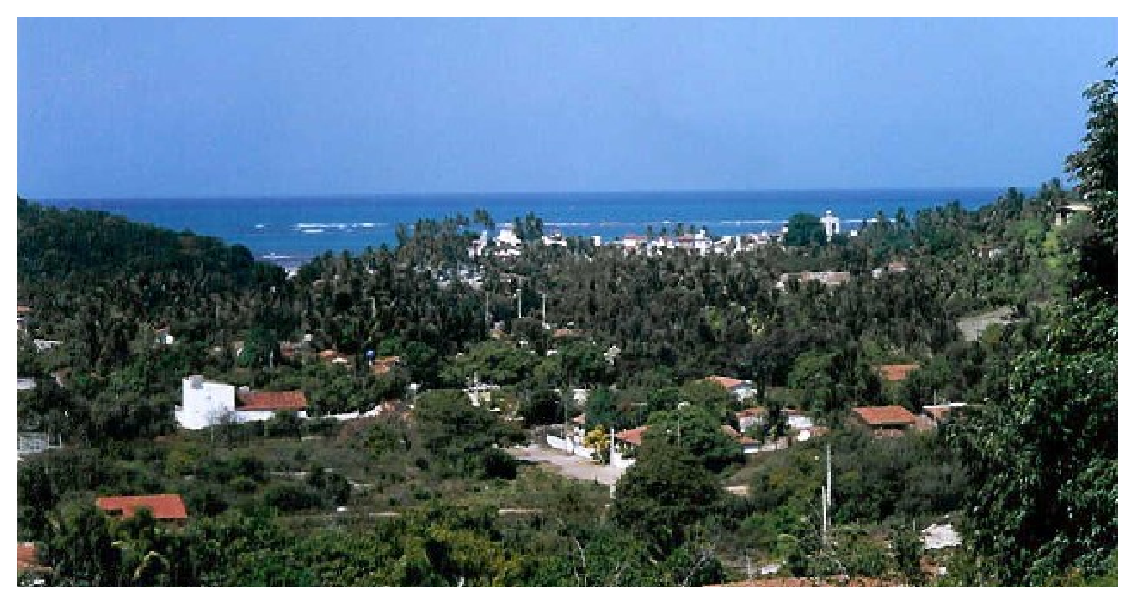
\includegraphics[width=0.75\linewidth]{textuais/04-problema/figuras/belmonte}}
\caption{Exemplo de imagem real}
\label{Fig:belmonte}
\end{center} \end{figure}

\subsection{Figuras sintéticas}
\label{Sec:figsinteticas}

As figuras sintéticas podem ser armazenadas em formato
\emph{pixel}-a-\emph{pixel}, como se fossem uma imagem, ou em
formato vetorial. No formato vetorial as primitivas que formam a
figura (linhas, textos, etc.) são descritas pelos parâmetros que as
caracterizam (ponto de início e fim, \emph{string} e posição do texto,
etc.). As figuras em formato vetorial são mais adequadas pois
usualmente correspondem a arquivos menores e a qualidade da imagem
não sofre perdas ao se aumentar ou diminuir o tamanho da figura.

Para inclusão no \LaTeX, os formatos PDF e EPS são os únicos que podem
representar figuras no formato vetorial. Nem toda figura salva nestes
formatos, entretanto, é necessariamente vetorial, pois tanto o PDF
quanto o EPS podem representar tanto figuras em formato
\emph{pixel}-a-\emph{pixel} quanto figuras em formato vetorial. Para
que sua figura seja vetorial, é necessário que o \emph{software} que a
gerou tenha a capacidade de produzi-las.

Para demonstrar a melhor qualidade das figuras em formato vetorial,
nas figuras \ref{Fig:bigvetorial} e \ref{Fig:bigbitmap} se mostra em
tamanho natural um mesmo diagrama nos formatos vetorial e de
\emph{pixels}. Nas figuras \ref{Fig:bigvetorialreduzida} e
\ref{Fig:bigbitmapreduzida} estas mesmas figuras são apresentadas
com uma redução de 50\%, utilizando o parâmetro \texttt{scale} do
\texttt{includegraphics}. Já nas figuras \ref{Fig:smallvetorial} e
\ref{Fig:smallbitmap} o diagrama original foi reduzido, de forma que
seu tamanho natural é menor. Nas figuras
\ref{Fig:smallvetorialampliada} e \ref{Fig:smallbitmapampliada}
este diagrama pequeno está aumentado de um fator arbitrário, calculado
pelo \texttt{includegraphics} para que a imagem ocupe toda a largura
da linha.

\begin{figure}[htbp!] \begin{center}
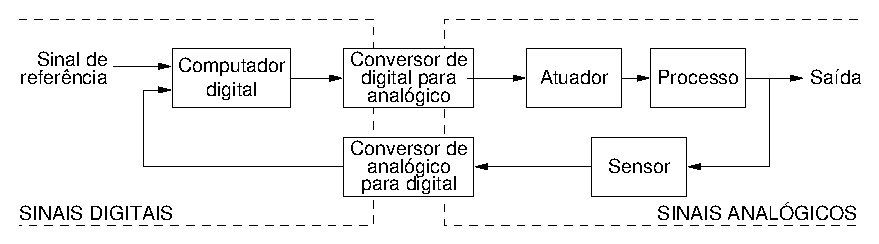
\includegraphics{textuais/04-problema/figuras/bigvetorial}
\caption{Figura vetorial grande em tamanho natural}
\vspace{6mm}
\label{Fig:bigvetorial}
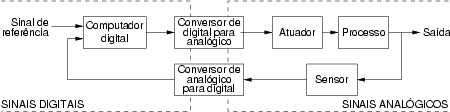
\includegraphics{textuais/04-problema/figuras/bigbitmap}
\caption{Figura \emph{pixel}-a-\emph{pixel} grande em tamanho natural}
\label{Fig:bigbitmap}
\vspace{6mm}
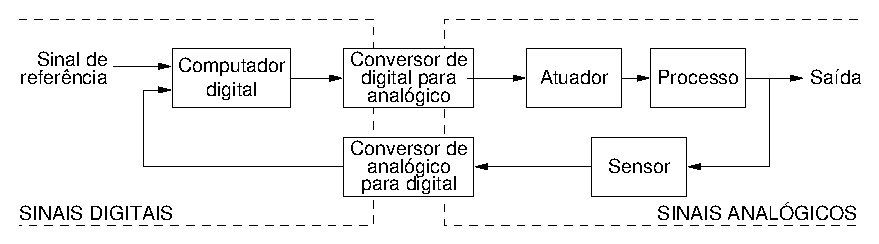
\includegraphics[scale=0.5]{textuais/04-problema/figuras/bigvetorial}
\caption{Figura vetorial grande em tamanho reduzido}
\label{Fig:bigvetorialreduzida}
\vspace{6mm}
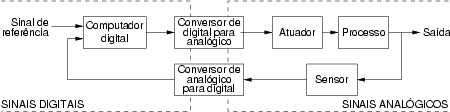
\includegraphics[scale=0.5]{textuais/04-problema/figuras/bigbitmap}
\caption{Figura \emph{pixel}-a-\emph{pixel} grande em tamanho reduzido}
\label{Fig:bigbitmapreduzida}
\end{center} \end{figure}

\begin{figure}[htbp!] \begin{center}
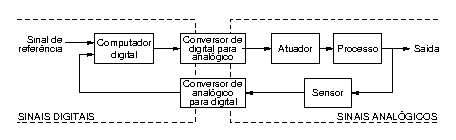
\includegraphics{textuais/04-problema/figuras/smallvetorial}
\caption{Figura vetorial pequena em tamanho natural}
\label{Fig:smallvetorial}
\vspace{6mm}
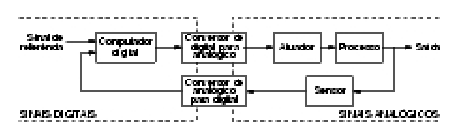
\includegraphics{textuais/04-problema/figuras/smallbitmap}
\caption{Figura \emph{pixel}-a-\emph{pixel} pequena em tamanho natural}
\label{Fig:smallbitmap}
\vspace{6mm}
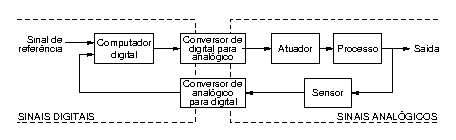
\includegraphics[width=\linewidth]{textuais/04-problema/figuras/smallvetorial}
\caption{Figura vetorial pequena em tamanho ampliado}
\label{Fig:smallvetorialampliada}
\vspace{6mm}
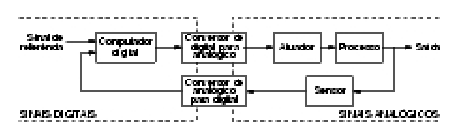
\includegraphics[width=\linewidth]{textuais/04-problema/figuras/smallbitmap}
\caption{Figura \emph{pixel}-a-\emph{pixel} pequena em tamanho ampliado}
\label{Fig:smallbitmapampliada}
\end{center} \end{figure}

Nota-se que no formato vetorial as
linhas mantêm a espessura mesmo quando se fazem
ampliações ou reduções. Já no formato de \emph{pixels}
as linhas ficam mais claras (cinzas, ao invés de pretas) após as
reduções e mais grossas após as ampliações, além de uma perda geral
de definição da imagem.

\section{Ferramentas para desenhos e esquemas}
\label{Sec:desenhos}

Existem diversas ferramentas para fazer desenhos, mas muitas delas
apenas salvam a figura gerada em formatos \emph{pixel}-a-\emph{pixel}.
No Unix, pode-se utilizar o \texttt{xfig}, que exporta imagens em
muitos formatos, inclusive nos vetoriais (PDF e EPS). Os diagramas das
figuras \ref{Fig:bigvetorial} a \ref{Fig:smallbitmapampliada} foram
desenhados e exportados no \texttt{xfig}. O arquivo fonte
correspondente é o \texttt{diagrama.fig}, no diretório
\texttt{figuras}.

A possibilidade de salvar figuras em modo vetorial impõe que alguns
recursos para desenho de imagens não sejam oferecidos. Um deles é o
desenho a mão-livre, já que seria impossível descrever a curva obtida
em termos de figuras geométricas básicas. Outro recurso inexistente é
o de preencher uma região com uma determinada cor. Esta última
limitação muitas vezes pode ser contornada utilizando-se a noção de
profundidade.  Por exemplo, para desenhar uma figura vazado e
preenchido de azul, pode-se desenhar a figura externa preenchido de
azul sobre o qual se desenha a figura interna preenchido de branco,
como mostram os exemplos da figura~\ref{Fig:circulo}.

\begin{figure}[htb] \begin{center}
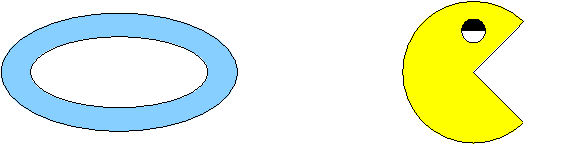
\includegraphics{textuais/04-problema/figuras/circulo}
\caption{Preenchimento de figuras utilizando diferentes profundidades}
\label{Fig:circulo}
\end{center} \end{figure}

A noção de profundidade no \texttt{xfig} foi exaustivamente utilizada
para desenhar os símbolos da UFRN e do PPgEEC que podem ser vistos na
página de rosto deste documento. Os arquivos \texttt{xfig}
correspondentes são \texttt{UFRN.fig} e \texttt{PPgEE.fig}. Ela também
pode ser utilizada para mesclar imagens com figuras sintéticas, como
na figura \ref{Fig:pensador} (veja arquivo \texttt{figuras/pensador.fig}).

\begin{figure}[htb] \begin{center}
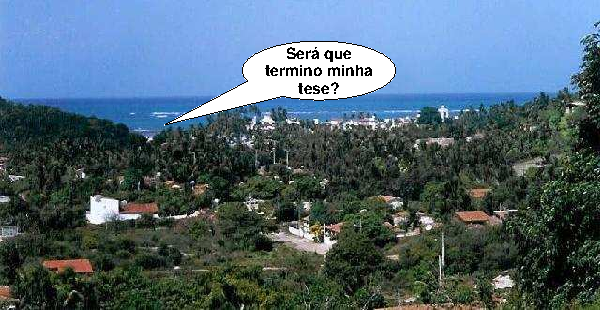
\includegraphics{textuais/04-problema/figuras/pensador}
\caption{Imagem mesclada com elementos sintéticos}
\label{Fig:pensador}
\end{center} \end{figure}

Outra possibilidade oferecida pelo \texttt{xfig} é a inclusão de comandos
\LaTeX\ dentro da figura. Para utilizar este recurso,
marque no \texttt{xfig} os textos que devem ser interpretados como
comandos \LaTeX\ com o \emph{flag} \texttt{special} e exporte a figura
no modo \emph{Combinado PS/Latex} ou \emph{Combinado PDF/Latex}. Veja
um exemplo na figura \ref{Fig:combinado}; note que o arquivo é incluído com
\verb|\input{}| e não com \verb|\includegraphics{}|.

% Note que foi redefinido um comando aqui no texto para ser incluído
% na figura. Isto é para evitar digitação de expressões LaTeX muito
% grandes dentro do xfig
\newcommand{\formulagrande}{$\frac{G_3G_4}{1-G_3G_4H_1}$}
\begin{figure}[htb] \begin{center}
%\input{textuais/04-problema/figuras/combinado.pstex_t} % Se usar latex
\input{textuais/04-problema/figuras/combinado.pdftex_t} % Se usar pdflatex
\caption{Figura incluindo comandos \LaTeX}
\label{Fig:combinado}
\end{center} \end{figure}

\section{Ferramentas para gráficos}
\label{Sec:graficos}

Gráficos devem ser gerados com aplicativos capazes de exportar o
resultado nos formatos EPS ou PDF, preferencialmente em formato
vetorial. Os conhecidos programas \emph{Scilab} e \emph{Matlab} têm
esta capacidade. Se você deseja algo mais simples, a ferramenta
\textit{GNUplot} é uma das mais utilizadas no Unix para a geração de
gráficos de funções matemáticas.

Uma vez gerados, gráficos são inseridos no texto tal como figuras. A
figura~\ref{fig:grafico} apresenta um gráfico gerado através do
comando de linha \texttt{gnuplot grafico.gnuplot}. Este arquivo
\texttt{grafico.gnuplot}, que contém uma série de comandos do
\textit{GNUplot}, está no diretório \texttt{figuras}.

\begin{figure}[htbp]
\centering
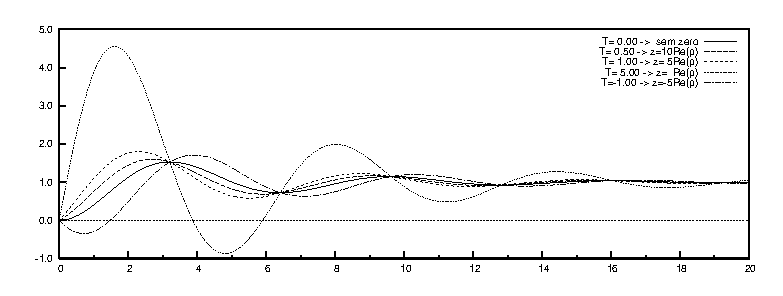
\includegraphics{textuais/04-problema/figuras/grafico}
\caption{Exemplo de gráfico de funções matemáticas}
\label{fig:grafico}
\end{figure}

\section{Conclusões}

Ferramentas de desenho capazes de gerar a saída em formato vetorial
são mais difíceis de usar e parecem ser dotadas de menos recursos do
que outras que só exportam seus resultados como imagens de
\emph{pixels}.  Isto se deve à necessidade de descrever todos os
elementos da imagem sob a forma de primitivas parametrizáveis para
permitir que elas sejam escaláveis à vontade e exportáveis para
qualquer formato desejado.

Entretanto, a qualidade visual das figuras obtidas e a sua
reusabilidade é muito maior. A comparação é aproximadamente a mesma
que a entre textos produzidos em \LaTeX\ e em editores gráficos. Desta
forma, na medida do possível, tente conjugar a escrita do documento
\LaTeX\ com a utilização de alguma ferramenta de desenho vetorial.

% LocalWords:  editadas PS
